% Slides: Geschichte des Internets

\begin{frame}
    \centering
    \begin{figure}[H]
        
\includegraphics[keepaspectratio, width=0.7\paperwidth, height=\paperheight]{Logos/LeeLogo.pdf}
    \end{figure}
    Informatik: Data Science und Sicherheit\\
    \emoji{globe-with-meridians} \textbf{Netzwerke: Geschichte des Internets}
\end{frame}

\begin{frame}{Die Anfänge: ARPANET und die 1960er Jahre}
    \begin{itemize}
        \item 1969: Erste Nachricht zwischen zwei Computern am \textbf{ARPANET}
        \item Ziel: Robustes, dezentrales Netzwerk, auch bei Ausfällen funktionsfähig
        \item Austausch von Informationen zwischen Universitäten und Forschungseinrichtungen
    \end{itemize}
    \begin{figure}[H]
        \centering
        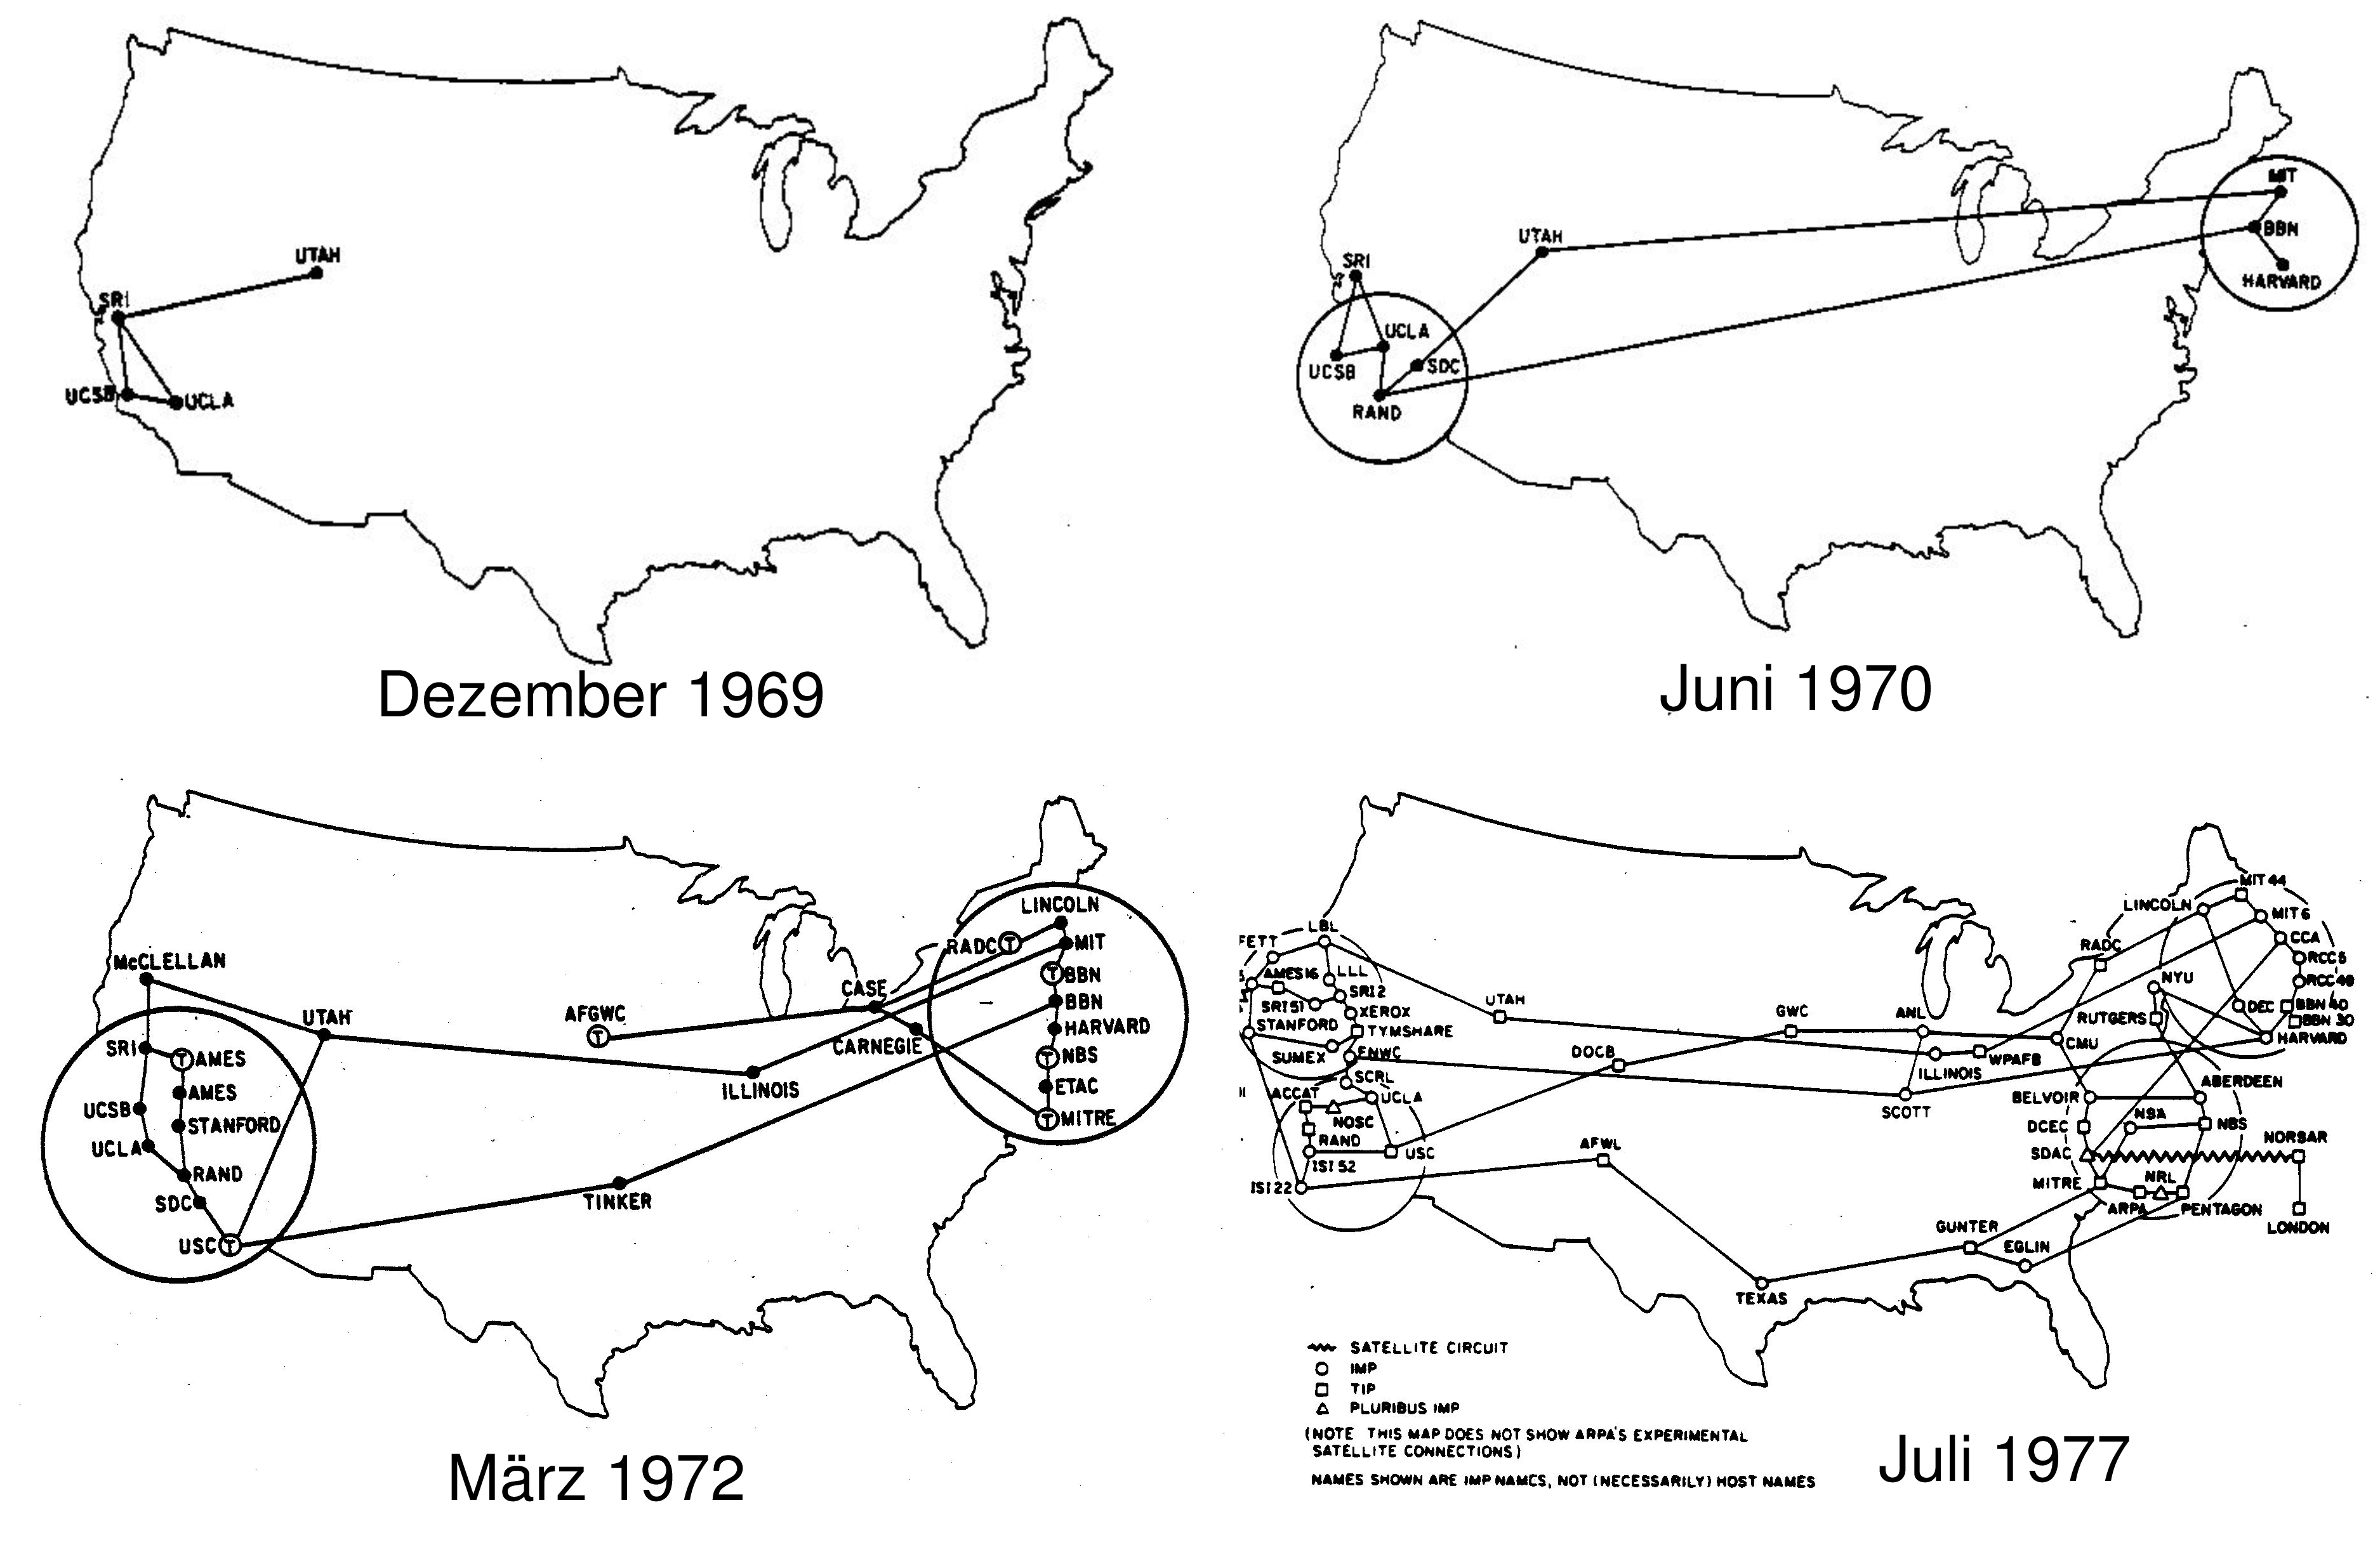
\includegraphics[width=0.7\linewidth]{Grundlagen_Info/07_Netzwerke/Figures/arpanet.png}
    \end{figure}
\end{frame}

\begin{frame}{Die Entwicklung von Protokollen: TCP/IP}
    \begin{itemize}
        \item 1983: Umstellung des ARPANET auf das \textbf{TCP/IP}-Protokoll
        \item Ermöglicht Kommunikation zwischen verschiedenen Netzwerken
        \item 1980er: Entstehung weiterer Netzwerke (CSNET, BITNET) und deren Zusammenschluss
    \end{itemize}
\end{frame}

\begin{frame}{Das WWW und die 1990er Jahre}
    \begin{itemize}
        \item 1990: Erfindung des World Wide Web (WWW) durch Tim Berners-Lee
        \item Einführung von HTML, HTTP und Hyperlinks
        \item 1991: WWW wird der Öffentlichkeit vorgestellt
        \item 1995: Kommerzielle Nutzung, Gründung von Amazon, eBay
    \end{itemize}
    \begin{figure}[H]
        \centering
        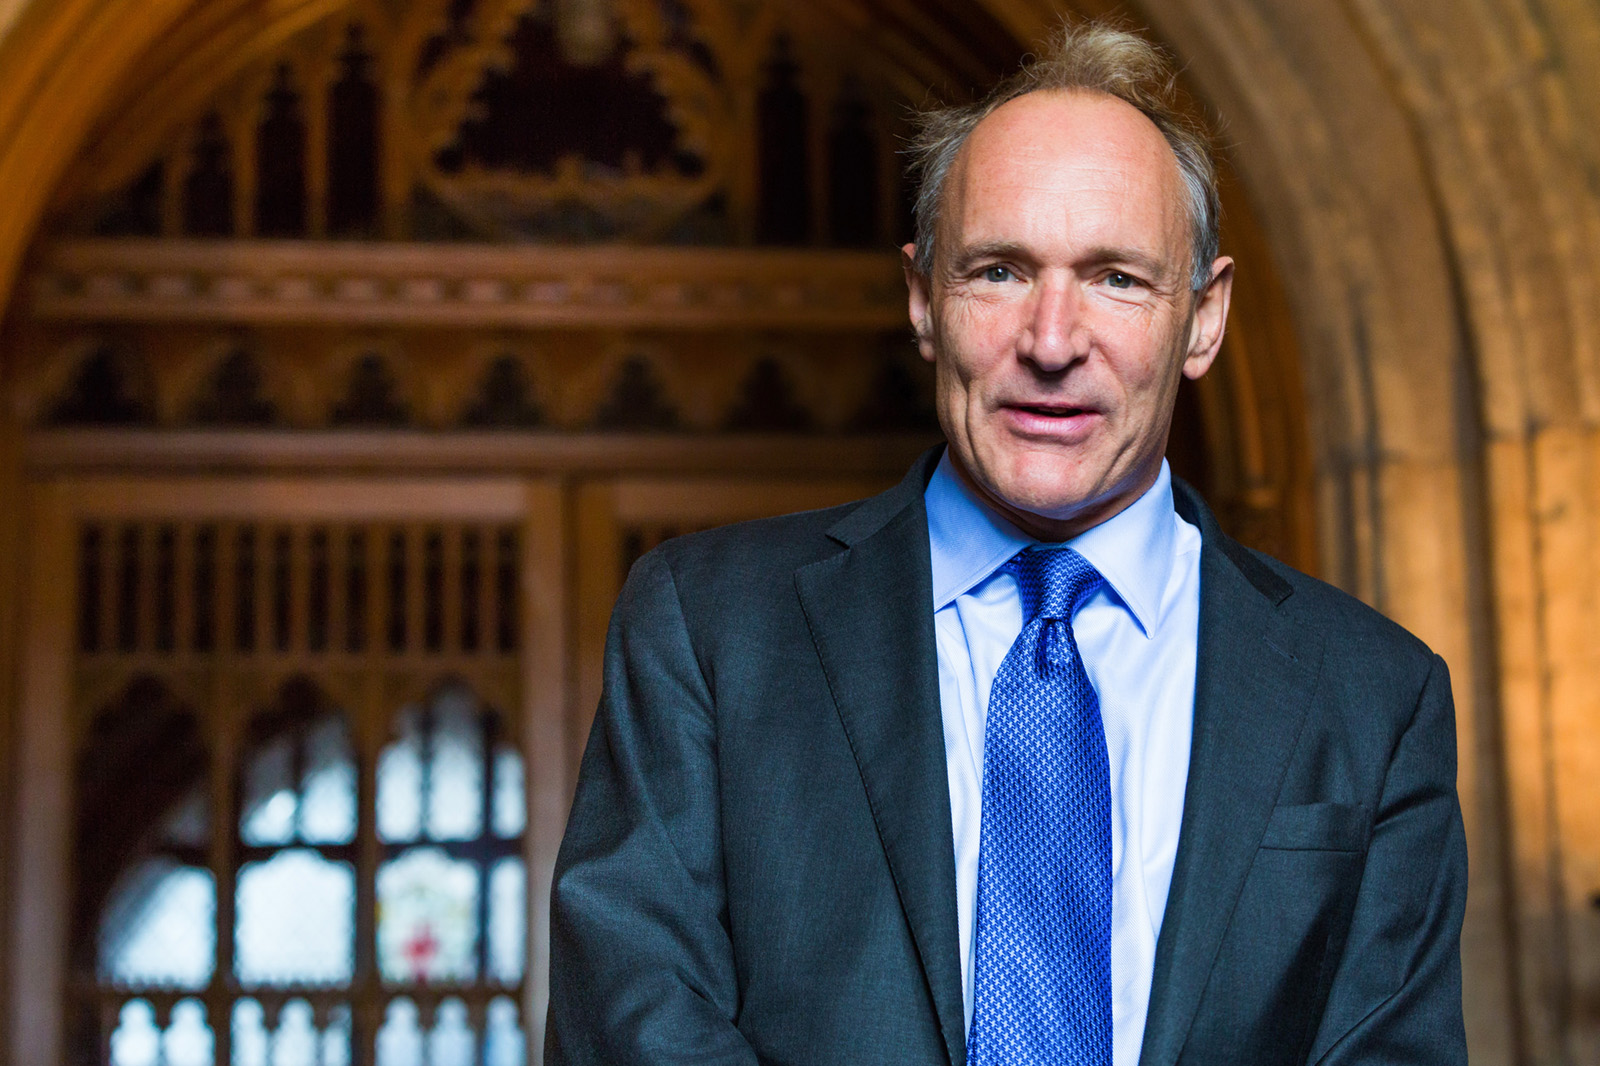
\includegraphics[width=0.5\linewidth]{Grundlagen_Info/07_Netzwerke/Figures/tim-berners-lee.jpg}
        \caption{Tim Berners-Lee, Erfinder des WWW}
    \end{figure}
\end{frame}

\begin{frame}{Das Internet im 21. Jahrhundert}
    \begin{itemize}
        \item 2000er: Verbreitung von schnellem Breitband-Internet, Aufstieg von Google, Facebook, YouTube
        \item Mobile Internet: Smartphones, ständiger Zugang zum Netz
        \item 2007: Einführung des iPhones, mobiles Internet wird allgegenwärtig: href{https://www.youtube.com/watch?v=MnrJzXM7a6o}{Video}
        \item Heute: Künstliche Intelligenz, 5G, weltweite Vernetzung
    \end{itemize}
\end{frame}

\begin{frame}{Internetnutzung weltweit}
    \begin{figure}[H]
        \centering
        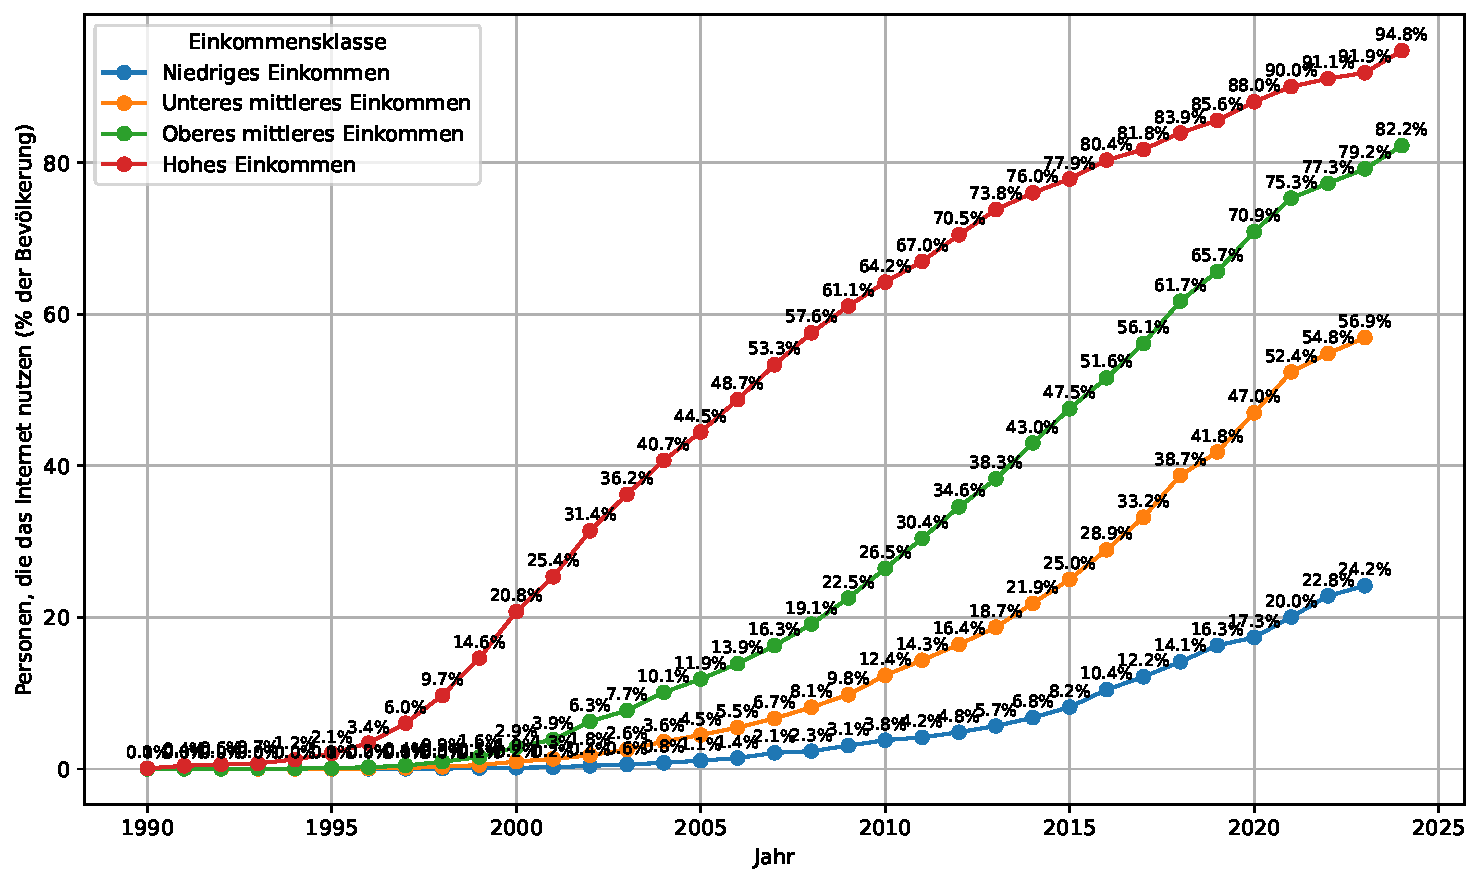
\includegraphics[width=\linewidth]{Grundlagen_Info/07_Netzwerke/Figures/internet_use_by_income_class}
    \end{figure}
\end{frame}

\begin{frame}{Internetnutzung weltweit}
    \begin{figure}[H]
        \centering
        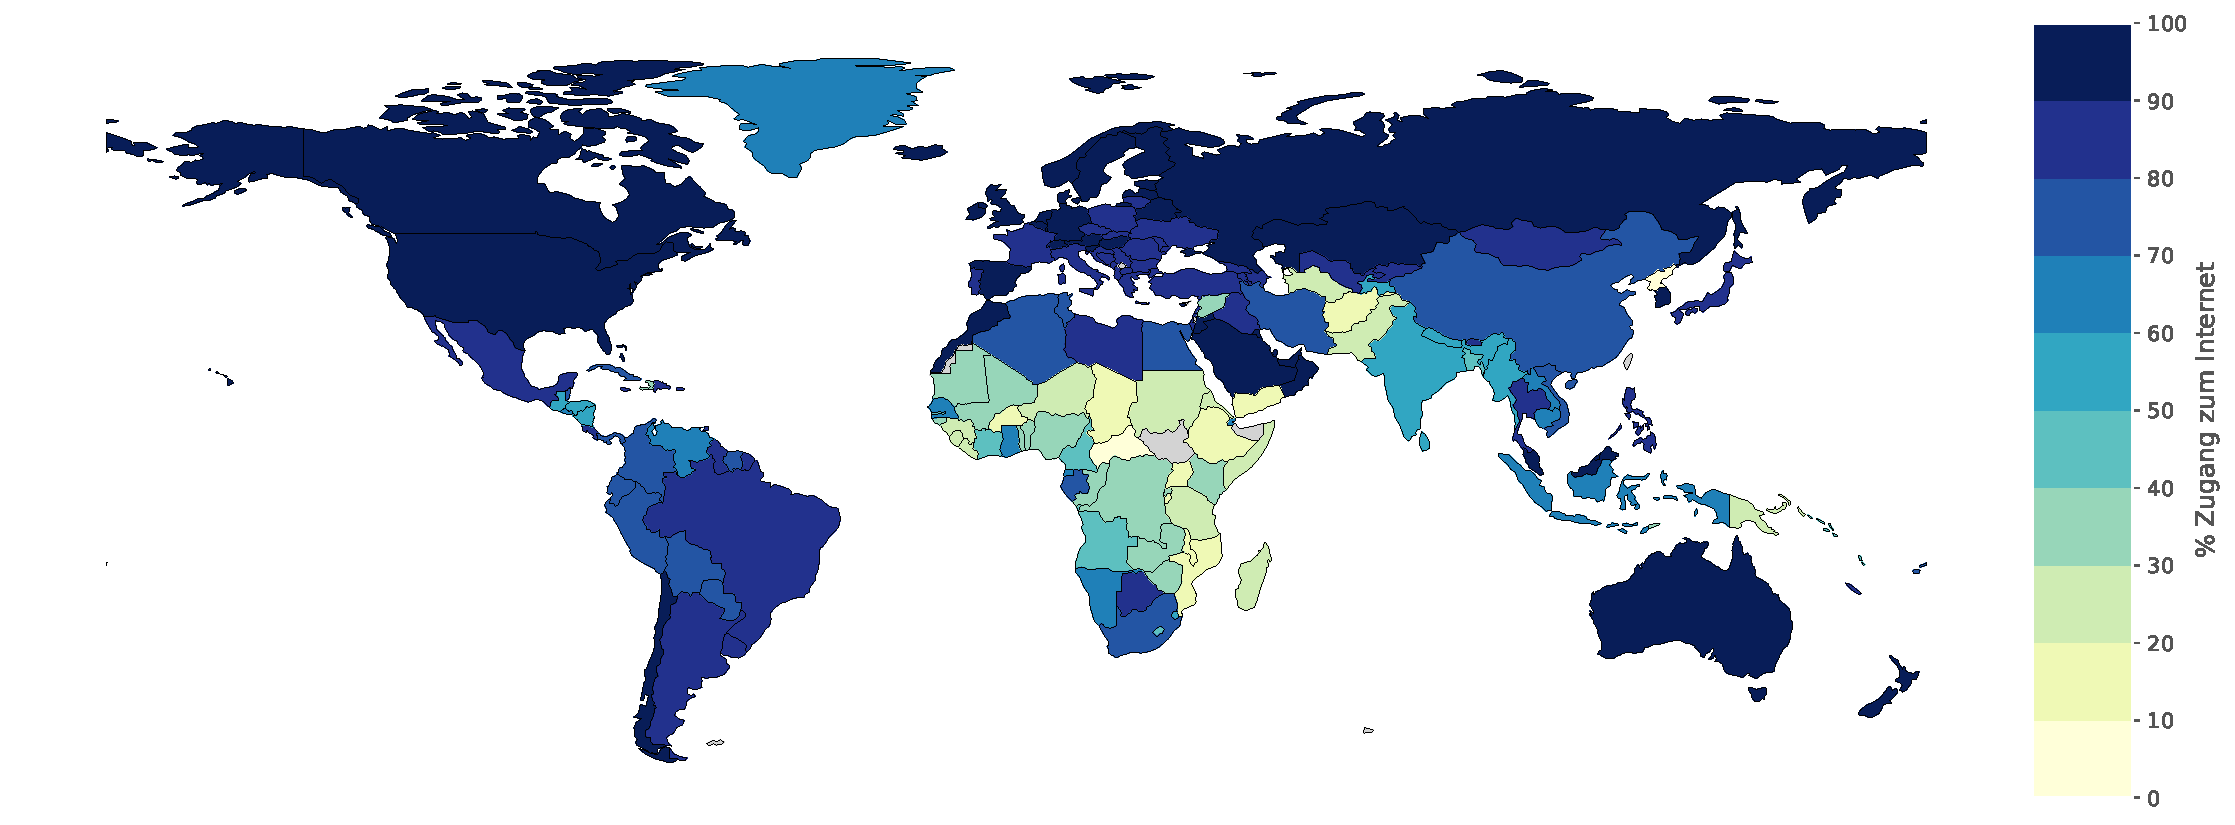
\includegraphics[width=\linewidth]{Grundlagen_Info/07_Netzwerke/Figures/internet_use_map_2024}
    \end{figure}
\end{frame}